% xelatex
% chktex-file 1
% chktex-file 3
% chktex-file 15
% chktex-file 17
% chktex-file 24
% chktex-file 25
% chktex-file 36
% chktex-file 45

\documentclass[10pt]{article}
\usepackage[top=20mm,bottom=20mm,left=20mm,right=20mm]{geometry}

\usepackage{xeCJK}
\usepackage[UTF8]{ctex}
 

\setlength{\parindent}{2em}

\usepackage{anyfontsize}
\usepackage{t1enc}
\usepackage{fontspec}

\usepackage{graphicx}
\usepackage{wrapfig}
\usepackage{float} %设置图片浮动位置的宏包
\usepackage{subfigure} %插入多图时用子图显示的宏包
\usepackage[justification=centering]{caption}
\usepackage[dvipsnames]{xcolor}
\usepackage{multirow}
\usepackage{booktabs}

\usepackage{amsmath}
\newcommand{\diff}{\mathrm{d}}
\newcommand{\lr}{\left(\right)}

\usepackage{siunitx}
\DeclareSIUnit{\hr}{hr}
\usepackage{textcomp} 


\usepackage{tikz}
\usepackage{tkz-euclide}
\usetikzlibrary{angles,calc, decorations.pathreplacing, arrows}

\usepackage[unicode, hidelinks]{hyperref}
\usepackage[all]{hypcap}

\usepackage{fancyhdr}
\usepackage{float}
\pagestyle{fancy}
\fancyhead[L]{冯翊展 2400017802}
\fancyhead[C]{}
\fancyhead[R]{\leftmark}

\title{\textbf{Quantitative Cell Biology Homework}}
\author{冯翊展 2400017802}
\date{Fall, 2025}

\begin{document}
\hypersetup{bookmarksnumbered=true,}

\maketitle

\begin{Large}
\tableofcontents
\end{Large}%
\pagebreak

\section{Homework 1 (10.15)}

\subsection{}
\subsubsection*{(a)}
$$j(r)=-\frac{I_0}{4\pi r^2}$$
量纲为``氧气量/（面积·时间）''，如$\qty{}{\kg\per\m\squared\per\s}$。

\subsubsection*{(b)}
$$j(r)=-\frac{I_0}{4\pi r^2} = -D\frac{\diff c(r)}{\diff r} \implies \frac{\diff c(r)}{\diff r} = \frac{I_0}{4\pi D r^2 } \implies \int \diff c(r) = \int \frac{I_0}{4\pi D r^2 } \diff r \implies c(r) = -\frac{I_0}{4\pi Dr}+C$$
由 $c(\infty)=c_0$：$C=c_0 \implies c(r) = c_0 - \frac{I_0}{4\pi Dr}$；
由 $c(R) = 0$：$c_0 = \frac{I_0}{4\pi DR} \implies D =\frac{I_0}{4\pi Dr}$。
故
$$c(r) = c_0-\frac{c_0R}{r} = c_0(1-\frac{R}{r})$$

\subsubsection*{(c)}
$$kR^2 = I_0 = 4\pi DRc_0 \implies R = \frac{4\pi D c_0}{k}$$

\subsection{}
\subsubsection*{(a)}
\begin{figure}[H]
    \centering
    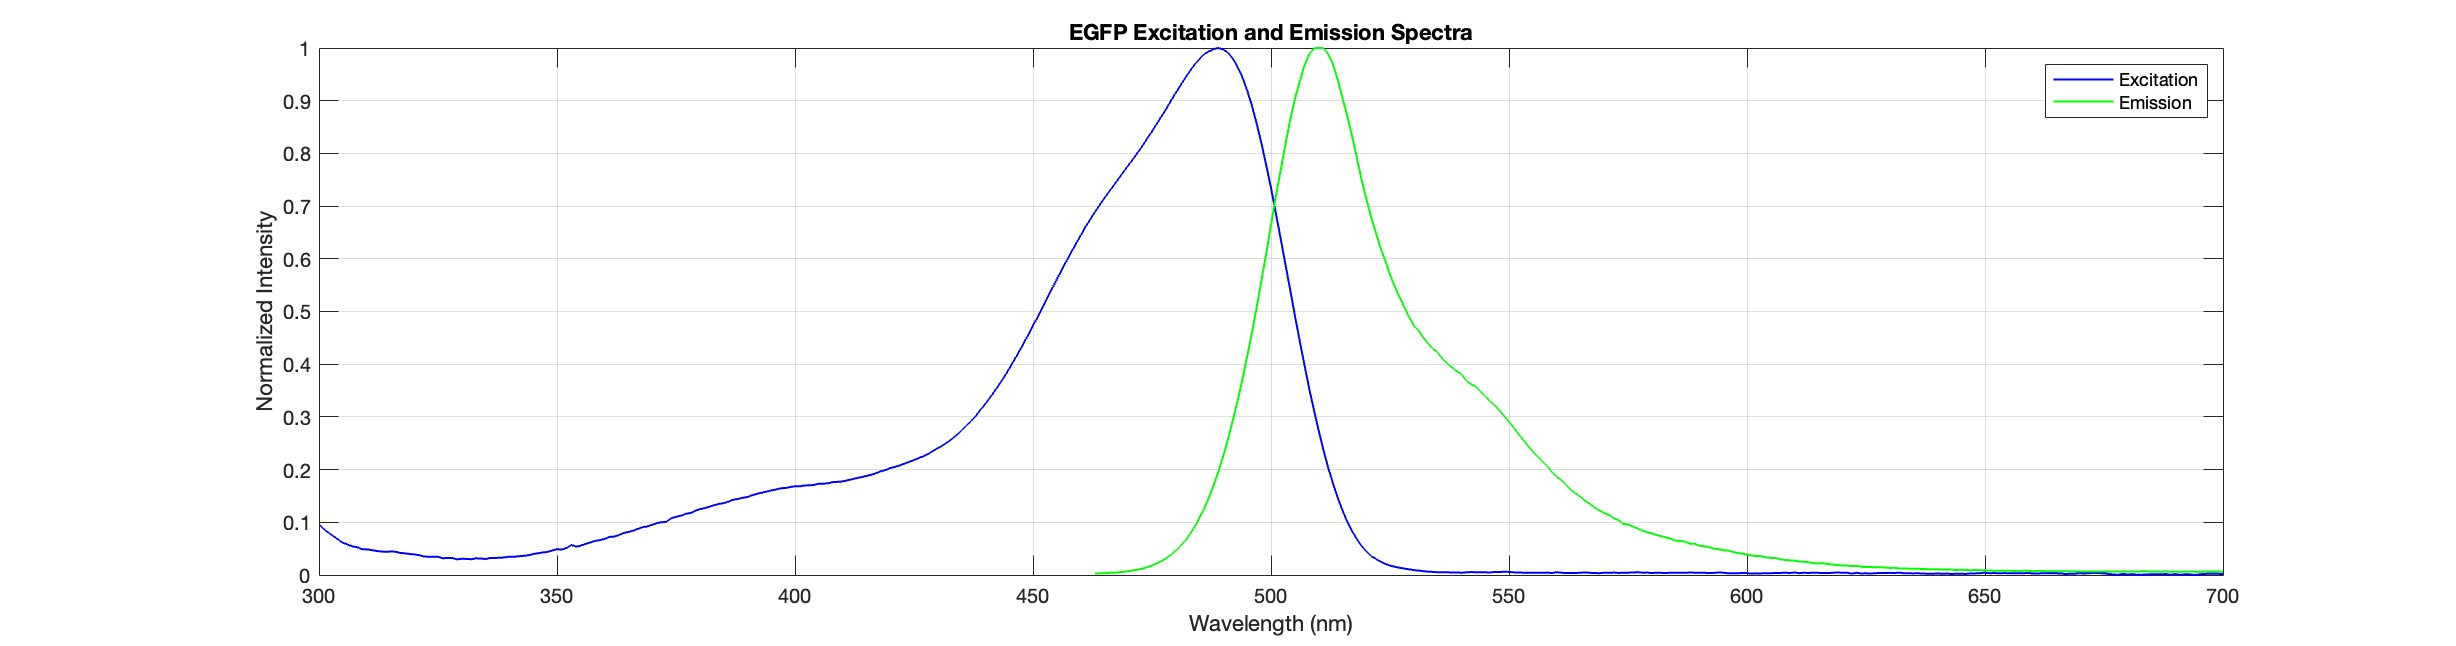
\includegraphics[width=0.75\linewidth]{Figures/EGFP Ex:Em Spectra.jpg}
    \captionof{figure}{EGFP Ex-Em Spectra}
\end{figure}

\subsubsection*{(b)}
\begin{figure}[H]
    \centering
    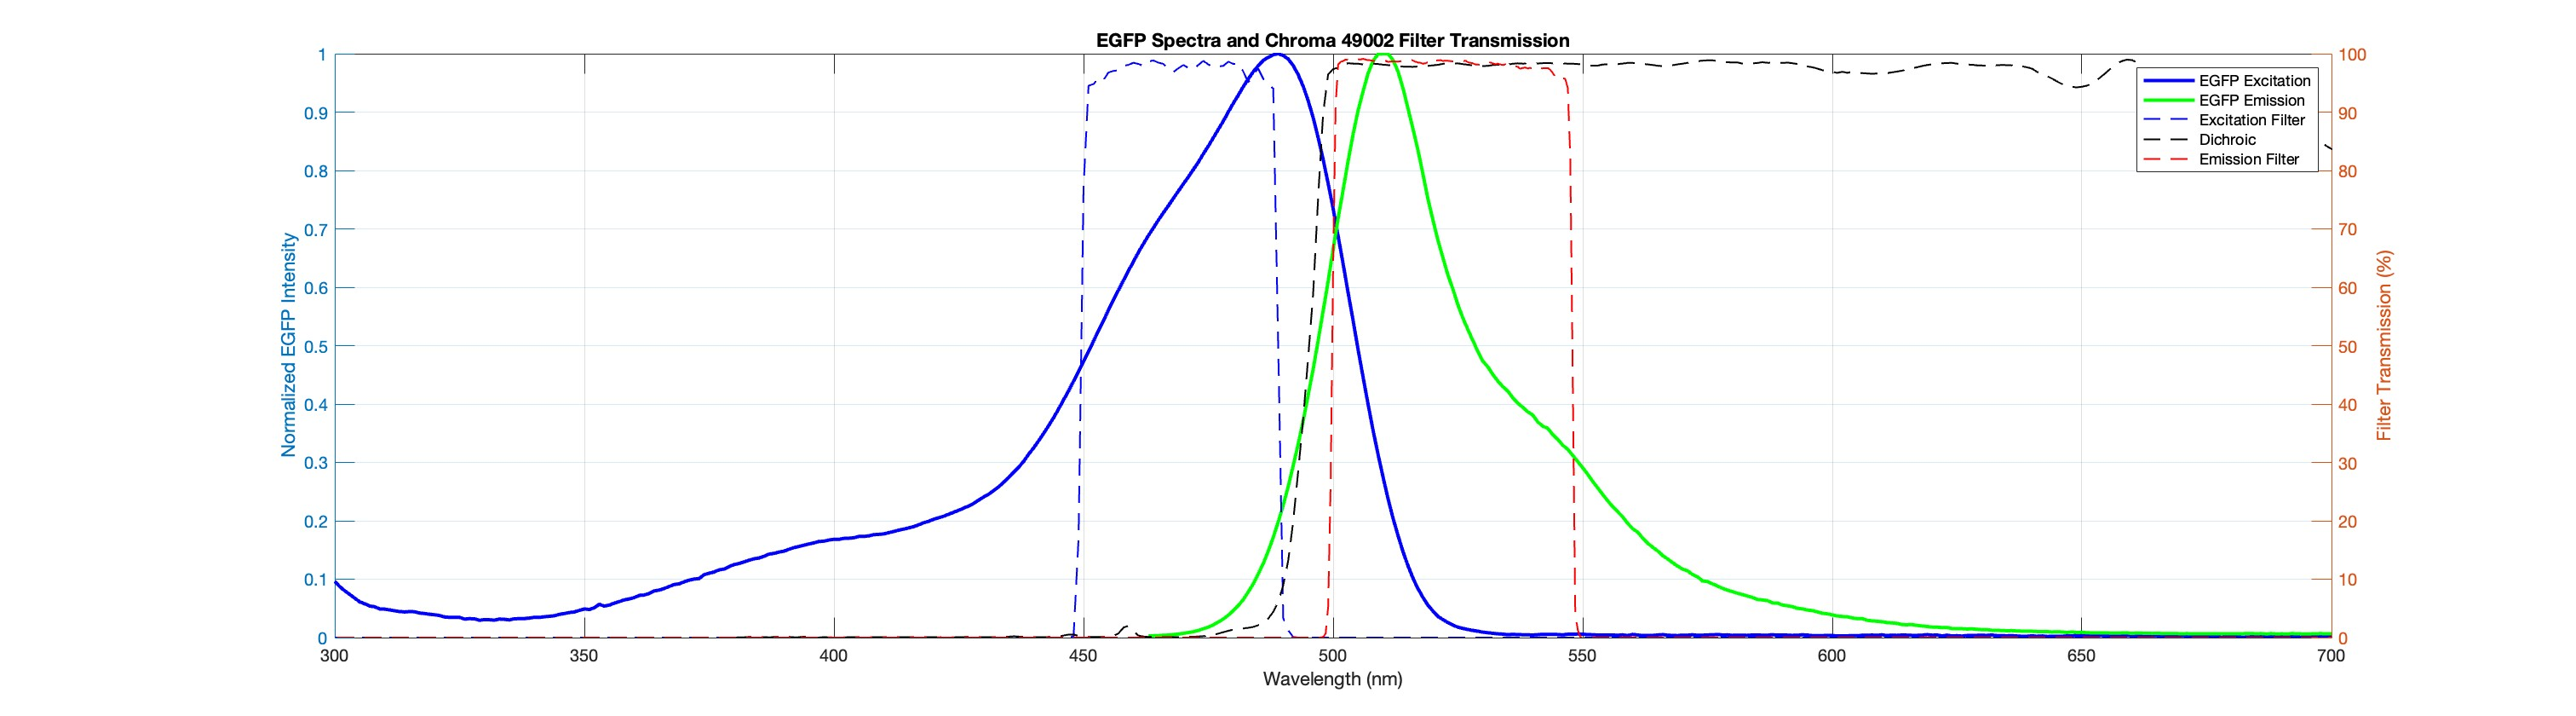
\includegraphics[width=0.75\linewidth]{Figures/EGFP.jpg}
    \captionof{figure}{EGFP Ex-Em Spectra and Filter Transmission}
\end{figure}

\subsubsection*{(c)}
\begin{figure}[H]
    \centering
    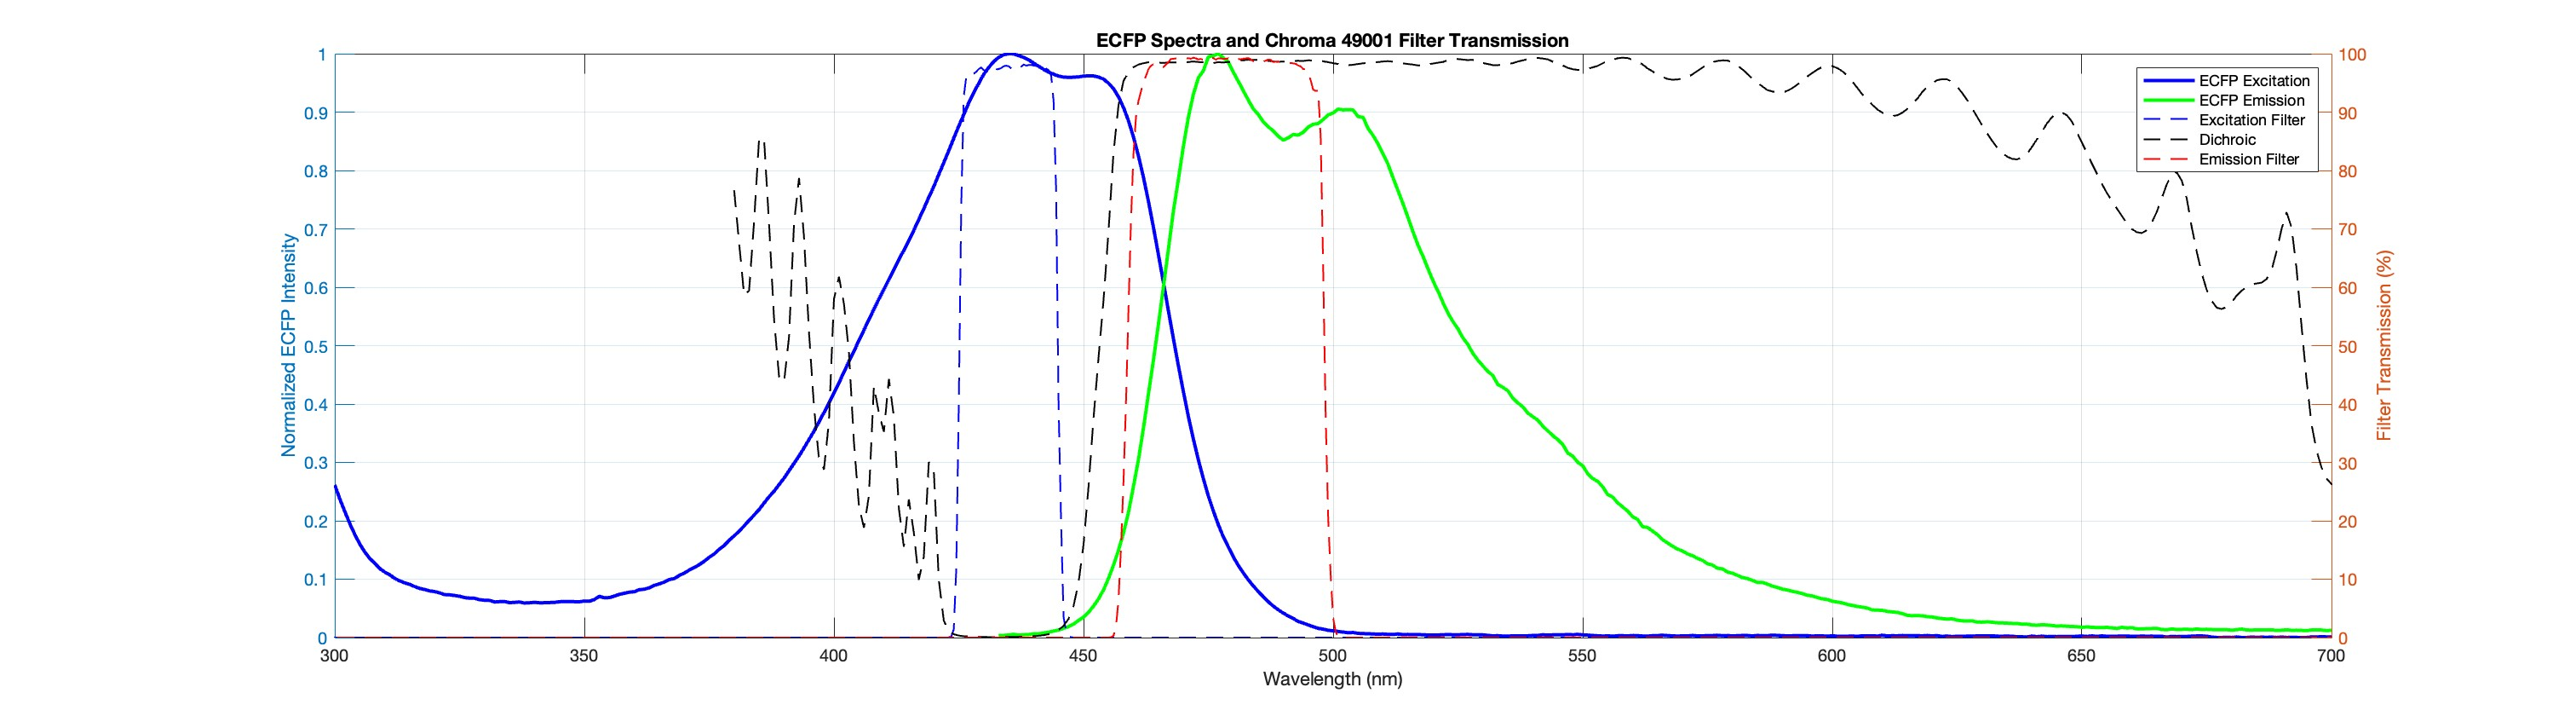
\includegraphics[width=0.75\linewidth]{Figures/ECFP.jpg}
    \captionof{figure}{EGFP Ex-Em Spectra and Filter Transmission}
\end{figure}

\subsubsection*{(d)}
不可行。一方面，使用EGFP通道观察时，EGFP激发滤光片（$470\pm \qty{20}{\nm}$）会激发一部分ECFP（$\sim \qty{470}{\nm}$），而ECFP发射峰部分延伸到了$\sim \qty{507}{\nm}$区域，这一部分进入了EGFP发射滤光片范围（$525\pm\qty{25}{\nm}$），因此ECFP信号会串扰进EGFP通道中，在观察内质网时细胞核也会部分亮起，无法区分。

另外，ECFP发射峰与EGFP激发峰有部分重叠，因此观察ECFP通道时ECFP激发光可能会交叉激发EGFP，造成进一步串扰。

\subsection{}
\subsubsection*{(a)}
适合使用转盘共聚焦显微镜（Spinning Disk Confocal Microscope, SDCM）：
\begin{itemize}
    \item 高时间分辨率，通过数千个微小的针孔同时扫描，成像速度极快，能够捕捉线粒体的动态变化。
    \item 提供亚细胞级分辨率，适合线粒体尺寸（约 $1\sim10$ \textmu m）。共聚焦技术可以排除焦平面外的模糊荧光，获得清晰的细胞内部图像，从而能精确地观察线粒体在细胞质中的三维分布和运动轨迹。
    \item 低光毒性，激光强度低，可在活细胞条件下长期观察。 
\end{itemize}

\subsubsection*{(b)}
适合使用冷冻电子显微镜（Cryo-EM）：
\begin{itemize}
    \item 病毒颗粒尺寸小于 $\qty{50}{\nm}$，这远远超出了光学显微镜的分辨率极限（$\sim \qty{200}{\nm}$）。电子显微镜利用电子束作为光源，其分辨率可达亚纳米级别，能够清晰地分辨病毒表面的蛋白尖刺、衣壳结构等精细形态。
    \item 冷冻电镜技术通过将样品在液态乙烷中快速冷冻，使其包裹在无定形冰中，最大限度地保留了样品的天然结构，避免化学固定或染色引起的结构损伤。
    \item 可以结合冷冻电子断层扫描（Cryo-ET），提供病毒在细胞表面附着时的三维空间结构信息。
\end{itemize}

\subsubsection*{(c)}
适合使用相差显微镜（Phase-contrast microscopy）：
\begin{itemize}
    \item 无需染色，利用光通过细胞内部不同结构（如细胞核、细胞质）时产生的相位差，并将其转换为肉眼可见的明暗对比度（振幅差），从而无损观察完全透明、未染色的活细胞。
    \item 可以增强透明细胞轮廓，清晰观察到细胞形态、铺展情况、伪足等结构以及细胞核的位置和大小。
    \item 可在活细胞条件下长期成像，无光毒性影响，且成本低，操作简便。
\end{itemize}

\subsection{}
\subsubsection*{1. 抗体和染料选择}

\capstartfalse
\begin{table}[h!]
\centering
\begin{tabular}{@{}ccc@{}}
\toprule
\textbf{目标结构} & \textbf{标记方式} & \textbf{激发/发射 ($\qty{}{\nm}$)} \\ \midrule
Golgi & 一抗（小鼠单抗 GM130） + 二抗（抗小鼠 Alexa Fluor 488） & 488 / 507 \\
Actin & Phalloidin 直接偶联荧光染料（Alexa Fluor 568） & 561 / 580 \\
Nucleus & DNA 染料（DAPI） & 358 / 461 \\ \bottomrule
\end{tabular}
\end{table}
\capstarttrue

\subsubsection*{2. 实验流程图}

\begin{center}
\begin{tikzpicture}[
    node distance=1cm and 1.5cm,
    process/.style={draw, rounded corners, minimum width=3.3cm, minimum height=1.8cm, align=center},
    >=stealth,            
    line width=1pt,      
    shorten >=3pt,      
    shorten <=3pt         
]


\node (cell)     [process] {培养细胞};
\node (fix)      [process, right=of cell] {固定\\(4\% PFA，$\qty{15}{\min}$)};
\node (perm)     [process, right=of fix] {透化\\(0.1\% Triton X-100，\\$\qty{10}{\min}$)};
\node (block)    [process, right=of perm] {封闭\\(BSA/血清，$\qty{60}{\min}$)};

\node (primary)  [process, below=of block] {一抗孵育\\(Golgi，过夜)};
\node (wash1)    [process, left=of primary] {PBS 洗涤 $3\times$};
\node (secondary)[process, left=of wash1] {二抗孵育\\(Alexa 488，$\qty{60}{\min}$)};
\node (wash2)    [process, left=of secondary] {PBS 洗涤 $3\times$};

\node (phalloidin) [process, below=of wash2] {Phalloidin\\(Actin-AF568)};
\node (wash3)    [process, right=of phalloidin] {PBS 洗涤 $3\times$};
\node (dapi)     [process, right=of wash3] {DAPI 染核\\（$\qty{5}{\min}$）};
\node (wash4)    [process, right=of dapi] {PBS 洗涤 $2\times$};

\node (image)    [process, below=of wash4] {封片并成像\\(蓝$\to$绿$\to$红)};

\draw[->] (cell) -- (fix);
\draw[->] (fix) -- (perm);
\draw[->] (perm) -- (block);

\draw[->] (block.south) to[out=-90, in=90] (primary.north);

\draw[->] (primary) -- (wash1);
\draw[->] (wash1) -- (secondary);
\draw[->] (secondary) -- (wash2);

\draw[->] (wash2.south) to[out=-90, in=90] (phalloidin.north);

\draw[->] (phalloidin) -- (wash3);
\draw[->] (wash3) -- (dapi);
\draw[->] (dapi) -- (wash4);

\draw[->] (wash4.south) to[out=-90, in=90] (image.north);

\end{tikzpicture}
\end{center}

\subsubsection*{3. 避免荧光信号串扰（Crosstalk）}

\begin{itemize}

    \item \textbf{荧光选择}：使用蓝（DAPI）、绿（Alexa 488）、红（Alexa 568）光谱间隔大的染料。
    \item \textbf{顺序标记}：先使用免疫染色Golgi，在直接染色Actin和Nucleus，避免二抗交叉反应。
    \item \textbf{成像顺序}：先拍 DAPI（蓝通道），再拍 Alexa 488（绿通道），最后拍 Alexa 568（红通道）。
    \item \textbf{光学优化}：使用窄带滤片，调节激光功率和曝光时间，降低光毒性，减少光谱重叠。
    \item \textbf{单标对照}：分别拍摄单标样品，验证各通道特异性，检测信号是否溢出到其他通道，用于后处理校正。

\end{itemize}

\subsection{}

与其说是一篇学术综述，这篇刊登于《Cell》的视角文章更像是一份宣告生物学研究范式即将彻底转变的``宣言书''。文章所描绘的``AI虚拟细胞''（AIVC）愿景，如同一场即将到来的科学海啸，引发了我们对未来科学探索模式的无限遐想。

文章最核心的突破性观点在于试图用``学习''取代``预设''，用``涌现''取代``还原''。传统的生物学模型，无论是微分方程还是基于主体的模拟，都建立在人类已有的、碎片化的知识之上，如同在黑暗中拿着手电筒，只能照亮已知的角落。而AIVC的提出，意味着我们试图创造一个会学习的数字生命。它通过吞噬海量的多模态数据——从基因序列到细胞影像——自主地构建起一套关于细胞运作的``统一语言''（通用表征）。这套语言可能超出我们当前的理解，但却能更本质、更全面地描述生命活动。这让我联想到AlphaFold在蛋白质结构预测上的革命：虽然并非完全理解物理化学原理，却能从序列中``领悟''结构。AIVC则将这一思想提升到了整个细胞甚至组织的尺度，其潜力无可估量。

毫无疑问，AIVC将带来科学发现范式的根本性逆转。文章指出，AIVC将从一个验证假设的工具转变为一个生成假设的引擎。这意味着，科学发现的主动权部分地从人类科学家移交给了AI。我们可以与AIVC进行对话，提出``如果……会怎样？''的开放式问题，让它在虚拟空间中执行数百万次在现实世界中成本高昂或伦理上不可行的实验，从而筛选出最有希望的研究路径。这就像拥有了一个不知疲倦、见多识广的研究助手，它能打破我们人类思维中的固有偏见和认知局限，揭示出那些隐藏在高维数据背后的、反直觉的生物学规律。未来的生物学实验室，或许将成为一个湿实验与干模拟紧密耦合、实时迭代的闭环系统。

与此同时，文章冷静地指出了通往这一宏伟愿景的道路上布满的荆棘。如何在黑箱的效力与白箱的理解之间取得平衡？ AIVC基于复杂的深度学习网络，其决策过程往往难以解释。当一个AIVC成功地预测了一种新的药物靶点或疾病机制时，我们能否完全信赖一个我们无法完全理解的``直觉''？这要求我们必须大力发展可解释AI，并建立全新的、侧重于生物学效用而不仅仅是统计指标的评估体系。

此外，文章也强调的开放科学与协作伦理至关重要。构建AIVC非一校一国之功，它需要全球科学界像完成人类基因组计划那样通力合作。数据、模型、基准必须开放共享，以避免数据封建和模型偏见。同时，我们必须警惕技术鸿沟，确保AIVC的发展能惠及全球所有人群，而非加剧健康不平等。当我们可以模拟个体患者的``数字孪生''时，数据隐私和伦理边界又该如何划定？这些问题已不再是遥远的哲学思辨，而是迫在眉睫的现实挑战。

通过这篇文章，我窥见了生命科学一个激动人心的未来。AIVC代表的不仅是一项技术革新，更是一种认识论的变革。它意味着我们开始尝试用生命自身的数据来理解生命，用系统整体的模拟来补充还原分析的局限。尽管前路漫漫，挑战重重，但这份蓝图足以让所有关心科学未来的人为之振奋。我们或许正站在一个历史性的拐点上，即将从一个``观察与描述生命''的时代，迈入一个``模拟与编程生命''的新纪元。而驱动这一切的，正是人工智能与生物学这场史诗般的相遇。

\newpage

\section{Homework 2 (10.29)}

\subsection{}
疏水效应的自由能成本与暴露的疏水表面积成正比，记比例常数为 $\gamma$。

初始状态下有 $N$ 个脂质分子分散在水中，每个脂质分子的疏水尾部完全暴露，总的疏水表面积为：
$$
A_{\text{separated}} = N \left( \pi d l + \frac{\pi d^2}{4} \right) = \pi N d \left( l + \frac{d}{4} \right).
$$
N个脂质分子最终形成双分子层，故
$$
\frac{1}{2}N\cdot \frac{\pi d^2}{4} = \frac{\pi D^2}{4} \implies D = d \sqrt{\frac{N}{2}}.
$$
最终状态下疏水尾部被埋藏在双分子层内部，但盘的边缘有疏水暴露，边缘表面积为：
$$
A_{\text{assembled}} = 2 \pi D l  = 2\pi \cdot d\sqrt{\frac{N}{2}}\cdot l = \pi d l \sqrt{2N}.
$$
因此组装过程中的疏水自由能变化为：
$$
\Delta G = \gamma\left(A_{\text{assembled}}-A_{\text{separated}}\right) =  \gamma \left[ \pi d l \sqrt{2N} - \pi N d \left( l + \frac{d}{4}\right)\right] =  \gamma \pi d \left[ l \sqrt{2 N} - N \left( l + \frac{d}{4} \right) \right].
$$
$N$充分大时，$\sqrt{N} \ll N$，故 $\Delta G < 0$，表明磷脂分子会自发聚集成双分子层。

\subsection{}
\subsubsection*{(a)}
对于长 $L$，半径为 $R$ 的圆柱形胶束，有以下约束条件：
$$
V = gv_0 = \pi R^2L, \ A = ga = 2\pi R L \implies R = \frac{2v_0}{a}.
$$
而 $l_0 < R$，故：
$$
\frac{1}{3} < \frac{v_0}{a\cdot l_0 } <\frac{1}{2}.
$$

对于厚 $L$ 的双分子平面层胶束，有以下约束条件：
$$
V =  gv_0 = A\cdot 2L = ga\cdot 2L \implies  L = \frac{v_0}{2a}.
$$
而 $ 2l_0 < L$，故：
$$
\frac{1}{2} < \frac{v_0}{a\cdot l_0} <1.
$$

\subsubsection*{(b)}
$$
\frac{v_0}{a\cdot l_0} = \frac{\qty{0.296}{\nm \cubed}}{ \qty{0.65}{\nm \squared} \cdot \qty{1.149}{\nm}} = 0.321 < \frac{1}{3}.
$$
故会形成球形胶束。胶束的直径为 $R = 3v_0/a = \qty{1.37}{\nm}$，故
$$
g = \frac{A}{a_0} = \frac{4\pi R ^2}{a_0} \approx 36.
$$
\subsubsection*{(c)}
溶血磷脂酰胆碱（lysophosphatidylcholines）具有单条烃链，疏水体积 $v_0$ 较小，导致 packing parameter $ \approx 0.3\sim0.4$，处于胶束范围（球形或圆柱形）。磷脂酰胆碱（phosphatidylcholines）具有两条烃链，$v_0$ 较大，packing parameter $ \approx 0.8\sim1$，处于双分子层范围。

\subsection{}
\subsubsection*{(a)}
考率半径为 $R$ 的细胞，表面积为 $A = 4\pi R^2$，体积为 $V = \frac{4}{3}\pi R^3$。假设 $c_\text{out} = 0$
$$
-V \frac{\diff c_\text{in}}{\diff t} = -\frac{\diff N}{\diff t} = jA = -P \Delta c\cdot A = -Pc_\text{in} \cdot A \implies \frac{\diff c_\text{in}}{\diff t} = \frac{PA}{V} c_\text{in}.
$$
故：
$$\tau = \frac{V}{PA} = \frac{\frac{4}{3}\pi R^3}{P\cdot 4 \pi R^2} = \frac{R}{3P}.
$$
取 $R = \qty{1}{\mu \m}$，$P = \qty{1e-10}{\m \per \s}$，则 $\tau \approx \qty{55.6}{\min}$。
对于磷酸化葡萄糖，$P' = P/100 = \qty{1e-12}{\m \per \s}$，则 $\tau' \approx \qty{92.6}{\hr}$，较普通葡萄糖增加100倍。

\subsubsection*{(b)}
求解方程：
$$
\frac{\diff c_\text{in}}{\diff t} = \frac{PA}{V} c_\text{in}.
$$
得到：
$$
c_\text{in}(t) = c_\text{in}(0)\cdot e^{\frac{t}{\tau}}, \tau = \frac{R}{3P}.
$$
与（a）一致。

\subsection{}
考虑Michaelis-Menten方程，毒素排出通量为：
$$
J=\frac{V_\text{max}C}{K_m+C}.
$$
毒素排出的速率为：
$$
\frac{\diff n}{\diff t}= - A J = -A \cdot \frac{V_\text{max}C}{K_m+C} = -A \cdot \frac{V_\text{max}\cdot n/V}{K_m+n/V} = -A\cdot \frac{V_\text{max}\cdot n}{K_mV+n}.
$$
代入 $A = \qty{1e-5}{\cm \squared}$，$V_\text{max} = \qty{1}{\pmol \per \cm \squared \per \hr}$，$K_m = \qty{1}{\mu M}$，$V = \qty{1e-9}{\cm \cubed}$得：
$$
\frac{\diff n}{\diff t} = - \frac{\qty{1e-5}{\pmol \per \hr}\cdot n}{\qty{1e-6}{\pmol}+n} \implies \diff t = - \frac{\qty{1e-6}{\pmol}+n}{\qty{1e-5}{\pmol \per \hr}\cdot n} \cdot \diff n.
$$
初态 $n_i = \qty{5}{\mu M} \cdot \qty{1e-9}{\cm \cubed} = \qty{5e-6}{\pmol} $，末态 $n_f = 0.01 \cdot n_i  = \qty{5e-8}{\pmol}$，故：
$$
t= \int_{n_i}^{n_f} - \frac{\qty{1e-6}{\pmol}+n}{\qty{1e-5}{\pmol \per \hr}\cdot n} \cdot \diff n \approx \qty{0.956}{\hr} \approx \qty{57.3}{\min}.
$$


\newpage

\section{Homework 3 (11.26)}

\subsection{} % 1. Physical Biology of the Cell 15.3
\subsubsection*{(a)}
根据质量作用定律，\(c_A(t)+c_B(t) = c_0\)，故：
\[
\frac{\diff c_A}{\diff t} = -k_+c_A + k_-c_B = -c_A (k_+ + k_-) + k_-c_0 = -(k_+ + k_-)\left(c_A- \frac{k_-c_0}{k_+ + k_-}\right).
\]
解这个微分方程得：
\begin{align*}
    \implies & \frac{\diff c_A}{\left(c_A- \frac{k_-c_0}{k_+ + k_-}\right)} = -(k_+ + k_-) \diff t \\
    \implies & \ln \left(c_A- \frac{k_-c_0}{k_+ + k_-}\right) = -(k_+ + k_-)t + C \\
    \implies & c_A(t) = C' e^{-(k_+ + k_-)t} + \frac{k_- c_0}{k_+ + k_-}.
\end{align*}
其中 \(C'\) 可以由 \(c_A(0)\) 确定：
\[
c_A(0) = c_0 = C' + \frac{k_- c_0}{k_+ + k_-} \implies C' = c_0 - \frac{k_- c_0}{k_+ + k_-}.
\]
因此：
\begin{align*}
    c_A(t) & = C' e^{-(k_+ + k_-)t} + \frac{k_- c_0}{k_+ + k_-} \\
    & = \left(c_0 - \frac{k_- c_0}{k_+ + k_-}\right) e^{-(k_+ + k_-)t} + \frac{k_- c_0}{k_+ + k_-} \\
    & = \frac{c_0}{k_+ + k_-} \left[k_+ e^{-(k_+ + k_-)t} + k_-\right], \\
    c_B(t) & = c_0 - c_A(t) \\ 
    & = \frac{k_+ c_0}{k_+ + k_-} \left[1 -  e^{-(k_+ + k_-)t} \right].
\end{align*}
作图如图~\ref{H3_1a}。对 \(t\) 取极限，有：
\begin{align*}
    & \lim_{t\to\infty} c_A(t) = \frac{k_-c_0}{k_+ + k_-}, \\
    & \lim_{t\to\infty} c_B(t) = \frac{k_+c_0}{k_+ + k_-}.
\end{align*}
故经过足够长的时间，
\[
\frac{c_A(\infty)}{c_B(\infty)} = \frac{k_-}{k_+}.
\]

\begin{figure}
    \centering
    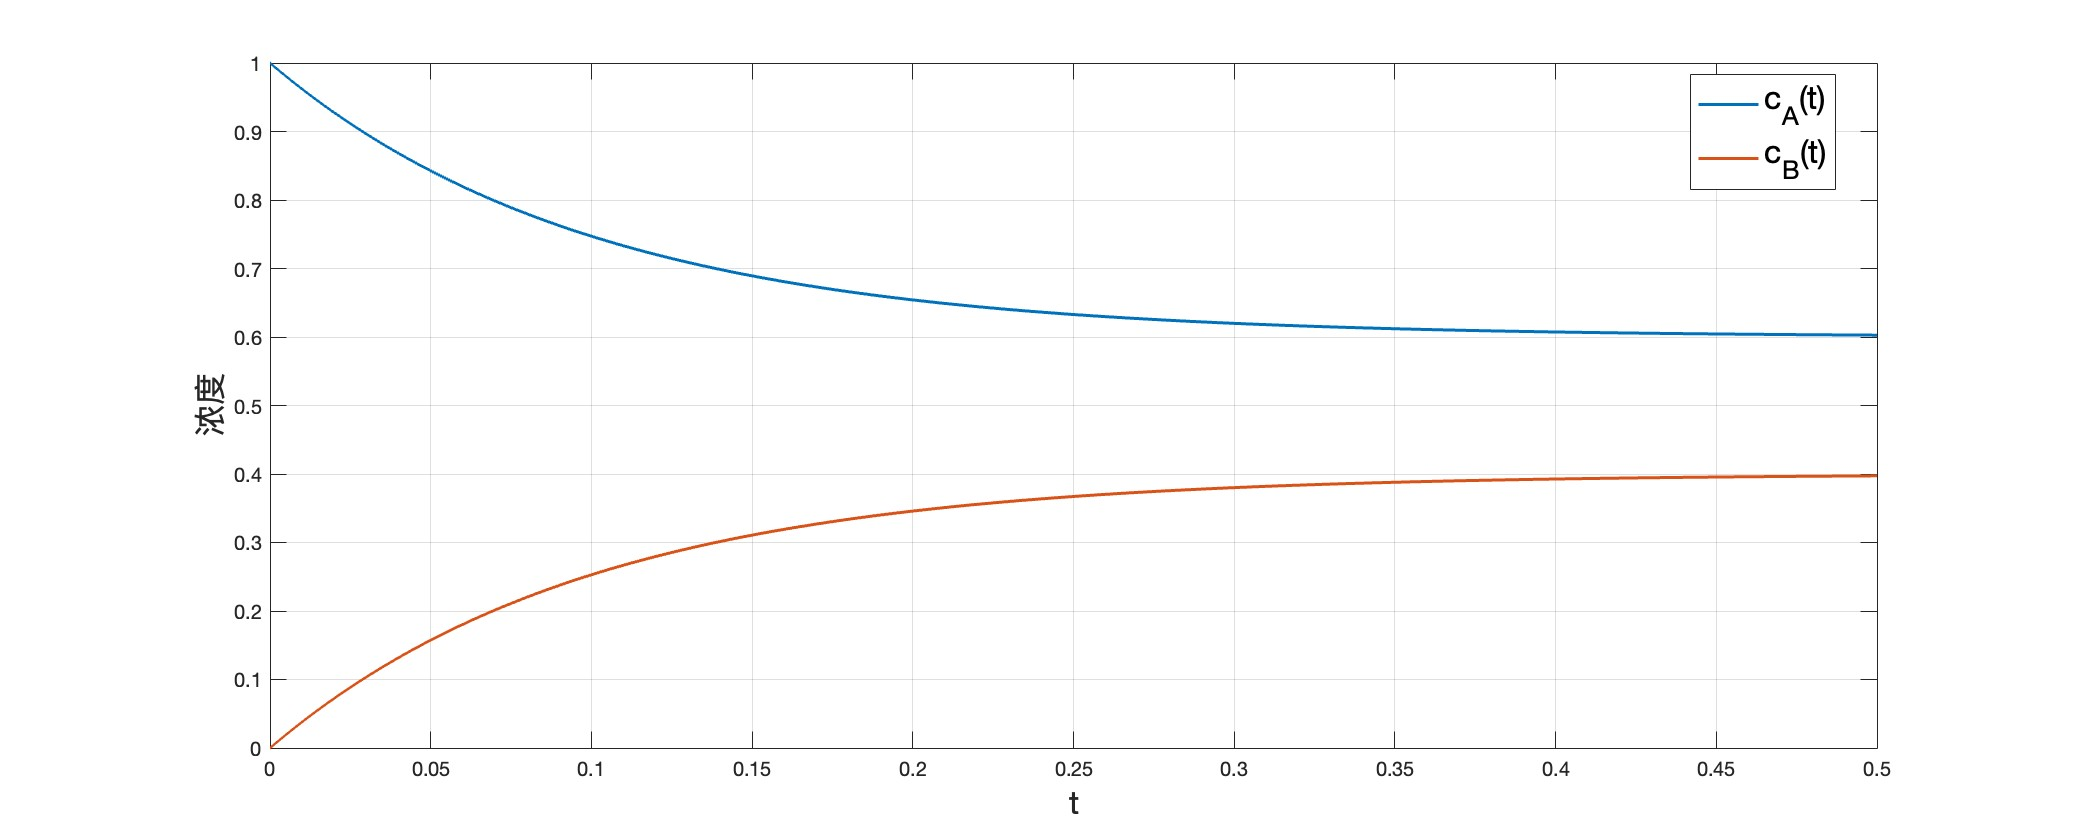
\includegraphics[width = 0.9\linewidth]{Figures/H3_1a.jpg}
    \captionof{figure}{\(c_A(t)\)与\(c_B(t)\)随时间变化，取\(c_0 = 1\)以及\(k_+ = 4, k_-=5\)}
    \label{H3_1a}
\end{figure}

\subsubsection*{(b)}

设 $A$ 表示通道关闭状态，$B$ 表示通道打开状态，稳态时满足：
\[
\frac{c_A(\infty)}{c_B{\infty}} = \frac{k_-}{k_+}.
\]
根据图 7.2A 中的电流记录，通道在关闭和开放状态下所处的时间几乎相等，因此：
\[
\frac{c_A(\infty)}{c_B{\infty}} = \frac{k_-}{k_+} \approx 1.
\]
同时在长约 \(\qty{80}{\ms}\) 的电流记录中观察到 \(20\) 次状态改变，因此可以估算状态弛豫时间约为：
\[
\tau = \frac{1}{k_+ + k_-} \approx \frac{\qty{80}{\ms}}{20} = \qty{4}{\ms}.
\]
假设初始时刻所有概率都集中在关闭状态，即 $c_A(0) = c_0 = 1$，则通道处于关闭和开放的概率随时间的函数为：
\begin{align*}
    c_A(t) & = \frac{1}{2} \left( e^{-t / \qty{4}{\ms}} + 1 \right),\\
    c_B(t) & = \frac{1}{2} \left( 1 - e^{-t / \qty{4}{\ms}} \right).   
\end{align*}
作图如图~\ref{H3_1b}。
\begin{figure}
    \centering
    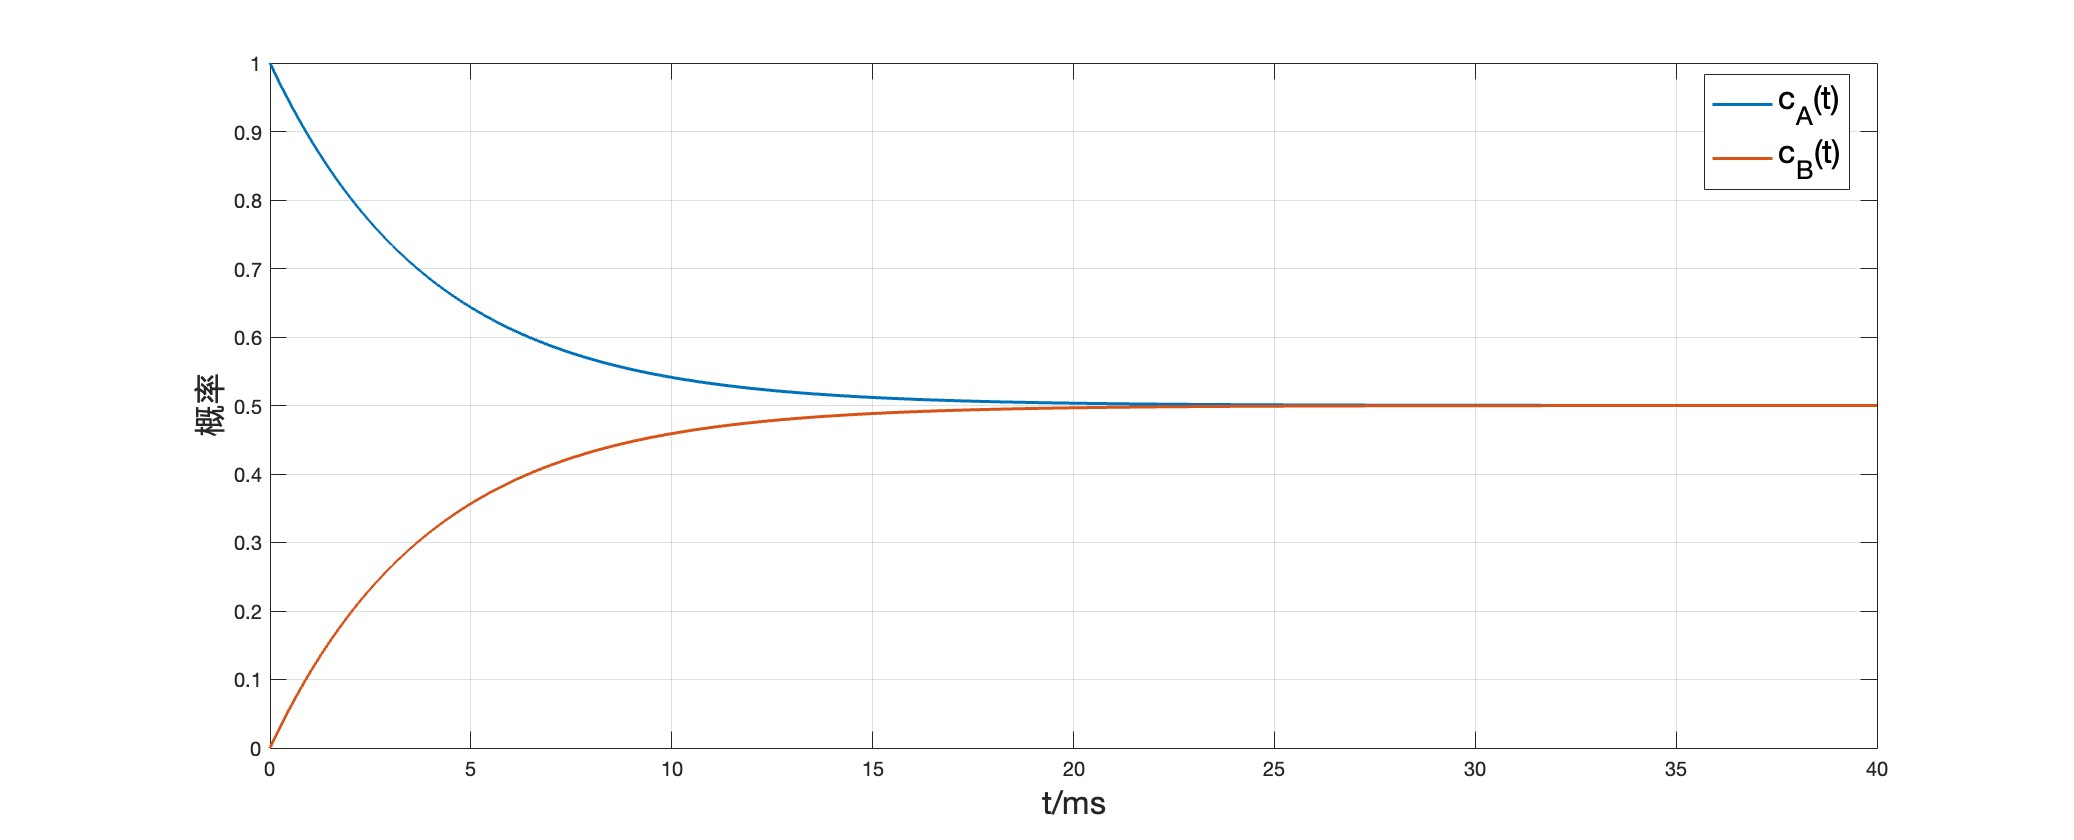
\includegraphics[width = 0.9\linewidth]{Figures/H3_1b.jpg}
    \captionof{figure}{通道关闭(A)和开放(B)概率随时间的变化}
    \label{H3_1b}
\end{figure}

\subsection{} % 2. Physical Biology of the Cell 15.7
\subsection*{(a)}
记 \(n_i\)，\(i = 1, 2, \ldots, N\)，表示每一个单体结合的 Kip3 数量，其中 \(N = L/l\) 表示单体数量，\(l\) 则是单个单体的长度。达到稳态时，第i个单体所集合的 Kip3 数量保持不变，即：
\[
k_{\text{bind}}\Delta t + n_{i-1} v \Delta t = n_i v\Delta t \implies n_i = n_{i-1} + \frac{k_{\text{bind}}}{v}.
\]
说明 \(n_i\) 构成等差数列，因此：
\[
n_i = i \cdot \frac{k_{\text{bind}}}{v}.
\]
符合观察到的线性增长。

\subsection*{(b)}
稳态下， Kip3 进入末端单体的通量为 \(Nk_{\text{bind}} = k_{\text{bind}}L/l \)，因此微管丝状体的解聚速率为：
\[
k_{\text{off}} = l \cdot Nk_{\text{bind}} = k_{\text{bind}} L.
\]
这个速率与微管丝状体长度成正比，与实验结果一致。在 \qty{3}{nM} 的 Kip3 浓度下，Kip3 的结合速率约为 
\[
k_{\text{bind}} \approx \frac{\qty{0.5}{\textmu\metre\per\minute}}{\qty{8}{\textmu\metre}} = \qty{0.0625}{\per\minute}.
\]
而 Kip3 浓度为 \(\qty{5.8}{nM}\)时，
\[
k_{\text{bind}} \approx \frac{\qty{2.0}{\textmu\metre\per\minute}}{\qty{6}{\textmu\metre}} = \qty{0.33}{\per\minute}.
\]
因此 \(k_{\text{bind}} \) 并不完全与 Kip3 的浓度成正比。

\subsection*{(c)}
设微管丝状体末端的聚合速率为 $k_{\text{on}}$，解聚速率为 $k_{\text{off}} = k_{\text{bind}}L$，则丝状体长度的变化速率为：
\[
\frac{\diff L(t)}{\diff t} = k_{\text{on}} - k_{\text{bind}}L.
\]
达到稳态时，丝状体长度保持不变，因此稳态长度为：
\[
L(\infty) = \frac{k_{\text{on}}}{k_{\text{bind}}}.
\]
在 \qty{3}{nM} Kip3 条件下，稳态长度 \(L(\infty) = \qty{16}{\textmu\metre}\)，该值与实际观测到的丝状体长度接近。

\subsection{} % 3. Molecular Biology of the Cell 15‐7
当激素的循环浓度为 \qty{1e-10}{\mol\per\litre} 时，
\[
\frac{[\text{R-H}]}{[\text{R}]_{\text{TOT}}} = \frac{\qty{1e-10}{\mol\per\litre}}{\qty{1e-10}{\mol\per\litre} + \qty{1e-8}{\mol\per\litre}} = 0.0099.
\]
即约有 1\% 的受体会与激素分子结合。若有一半的受体会结合激素分子，则
\[
\frac{[\mathrm{R\!-\!H}]}{[\mathrm{R}]_{\mathrm{TOT}}} = \frac{[\text{H}]}{[\text{H}] + \qty{1e-8}{\mol\per\litre}} = 0.5 \implies [\text{H}] = \qty{1e-8}{\mol\per\litre}.
\]
即激素浓度需要增加 100 倍才能引发有效的生理反应。

\subsection{} % 4. Molecular Biology of the Cell 15‐14
磷酸化激酶（PhK）整合了 cAMP 与 Ca\(^{2+}\) 两条信号通路，让两种输入同时作用在同一个全酶复合体上，共同把催化亚基推向活化构象。每一次磷酸化事件与每一个 Ca\(^{2+}\) 结合都提供一小步的变构动力，使活性与输入呈梯度、可叠加且具协同效应：只有 cAMP/PKA 或只有 Ca\(^{2+}\) 时为部分激活，两者同时存在时达到最大激活，这种``同位整合''的设计确保糖原分解在最需要时最强。同时，Ca\(^{2+}\) 信号起效快、短暂，而 PKA 磷酸化则更持久，直到被蛋白磷酸酶去磷酸化为止。如此 PhK 实现将两路激素信息汇总为单一输出，按需驱动糖原分解与葡萄糖输出。

\subsection{} % 5. Molecular Biology of the Cell 15‐15
个体细胞的``全或无''响应与群体的梯度响应并不矛盾。群体的梯度响应并非源于所有细胞的部分激活，而是由于群体中每个细胞具有略微不同的激活阈值，随着孕酮浓度升高，达到其阈值并完全激活的细胞比例逐渐增加，从而在宏观上形成了梯度剂量效应曲线。

在个体水平上，由于信号通路中存在正反馈循环（如激活的MAPK可以进一步增强上游信号的活性），MAP激酶模块相当于一个具有双稳态特性的生物化学开关。当孕酮信号低于某个临界阈值时，系统稳定在``关闭''状态（MAPK未激活）；一旦孕酮信号超过这个阈值，正反馈机制会将系统迅速且不可逆地推向另一个稳定的``开启''状态（MAPK完全激活）；而稳定的中间状态并不存在。因此，单个细胞的响应类似数字信号（全开或全关），导致在显微镜下卵母细胞要么出现白色斑点（完全激活），要么没有。

在群体水平上，细胞间的异质性，如信号蛋白（Mos, MEK, MAPK）表达量的微小差异，抑制因子或磷酸酶水平的差异以及细胞大小、代谢状态和细胞周期的微小不同，都会导致每个卵母细胞拥有略微不同的孕酮激活阈值。这导致激活阈值存在一个统计分布，群体响应实际上是不同阈值细胞比例变化的宏观体现。因此随着孕酮浓度升高，完全激活的细胞比例逐渐增加，微观层面的数字信号在宏观上反映为梯度响应的模拟信号。

\newpage

\section{Homework 4 (12.3)}

\subsection{}
选(b)：``G\(\beta\gamma\) 激活交配反应，而与 G\(\alpha\) 结合时受抑制''。

对照表中表型：
\begin{itemize}
    \item \(\alpha\)缺失：在无信息素时就出现生长停滞+交配反应，构成性激活，说明只要\(\beta \gamma\)游离即可启动通路；若由 G\(\alpha\) 激活则应在 \(\alpha\) 缺失时失活，故排除 (a)(e)。
    \item \(\beta\) 或 \(\gamma\) 缺失：即使加信息素也正常生长、无交配反应（不育），说明没有完整的 G\(\beta\gamma\)就不能激活通路，支持 (b)；若 ``G\(\alpha\) 或 G\(\beta\gamma\) 任一都能激活''，则 \(\beta\) 缺失应仍可由 G\(\alpha\) 激活，与事实相反，排除 (c)。
    \item 双缺失组合（\(\alpha+\beta\)、\(\alpha+\gamma\)、\(\beta+\gamma\)）：均表现为不育，与``需要 \(\beta \gamma\) 才能激活''一致；若三聚体本身有活性或需三聚体才能抑制，则应出现与野生型不同的无信息素表型，排除 (d)。
\end{itemize}
综上， 只有(b) 与所有突变体表型完全一致：野生型在无信息素时三聚体存在，G\(\alpha\) 抑制 G\(\beta \gamma\)；受体被信息素激活后，G\(\alpha\)·GTP 与 G\(\beta\gamma\) 解离，游离的 G\(\beta\gamma\) 启动下游（MAPK），导致生长停滞与交配反应。

\subsection{}
\subsection*{A.}
蛋白质 A 和 D 参与并促进 DNA 合成。只保留 A 结合位点的受体（突变体 2）能产生约 50\% 的最大 DNA 合成水平，只保留 D 结合位点的受体（突变体 5）也能产生约 50\% 的最大水平；而当 A 与 D 都能结合时（突变体 6），DNA 合成恢复到接近 100\% 的最大值。与完全不能结合任何蛋白质的突变体 9（几乎无 DNA 合成）相比，可以看出 A 和 D 的存在显著提高了 DNA 合成，因此 A 和 D 是促进 DNA 合成的蛋白质。

\subsection*{B.}
蛋白质 B 抑制 DNA 合成。只保留 D 结合位点的受体（突变体 5）可产生约 50\% 的最大 DNA 合成，而当 B 与 D 同时能结合时（突变体 7），DNA 合成水平下降到约 15\%。此外，只保留 B 结合位点的受体（突变体 3）仅略高于背景水平（突变体 9）。因此可以判断 B 会拮抗 D 的促进作用，从而起到抑制 DNA 合成的作用。

\subsection*{C.}
蛋白质 C 在本实验中没有可检测到的作用。只保留 C 结合位点的受体（突变体 4）产生的 DNA 合成水平与完全不能结合任何蛋白质的突变体 9 相近，接近背景；当 C 与 D 同时存在时（突变体 8），其 DNA 合成水平与只含 D 的突变体 5 相近（约 50\%），说明 C 的有无并不影响 D 的促进作用。因此 C 对 DNA 合成没有明显贡献。

\subsection{}
\begin{itemize}
    \item Rhodopsin 视紫质\\
    英文页面：https://en.wikipedia.org/wiki/Rhodopsin \\
    中文页面：\href{https://zh.wikipedia.org/wiki/%E8%A7%86%E7%B4%AB%E8%B4%A8}{https://zh.wikipedia.org/wiki/视紫质} \\
    大幅度扩充了中文页面的内容

    \item Second messenger system 第二信使系统\\
    英文页面：https://en.wikipedia.org/wiki/Second\_messenger\_system \\
    中文页面：\href{https://zh.wikipedia.org/wiki/%E7%AC%AC%E4%BA%8C%E4%BF%A1%E4%BD%BF%E7%B3%BB%E7%BB%9F}{https://zh.wikipedia.org/wiki/第二信使系统} \\
    大幅度扩充了中文页面的内容

    \item GCaMP\\
    英文页面：https://en.wikipedia.org/wiki/GCaMP \\
    中文页面：https://zh.wikipedia.org/wiki/GCaMP \\
    新建了中文页面并翻译了英文页面内容
\end{itemize}

\newpage

\section{Homework 5 (12.17)}

\subsection{} % Molecular Biology of the Cell 17-13

\begin{figure}[H]
    \centering
    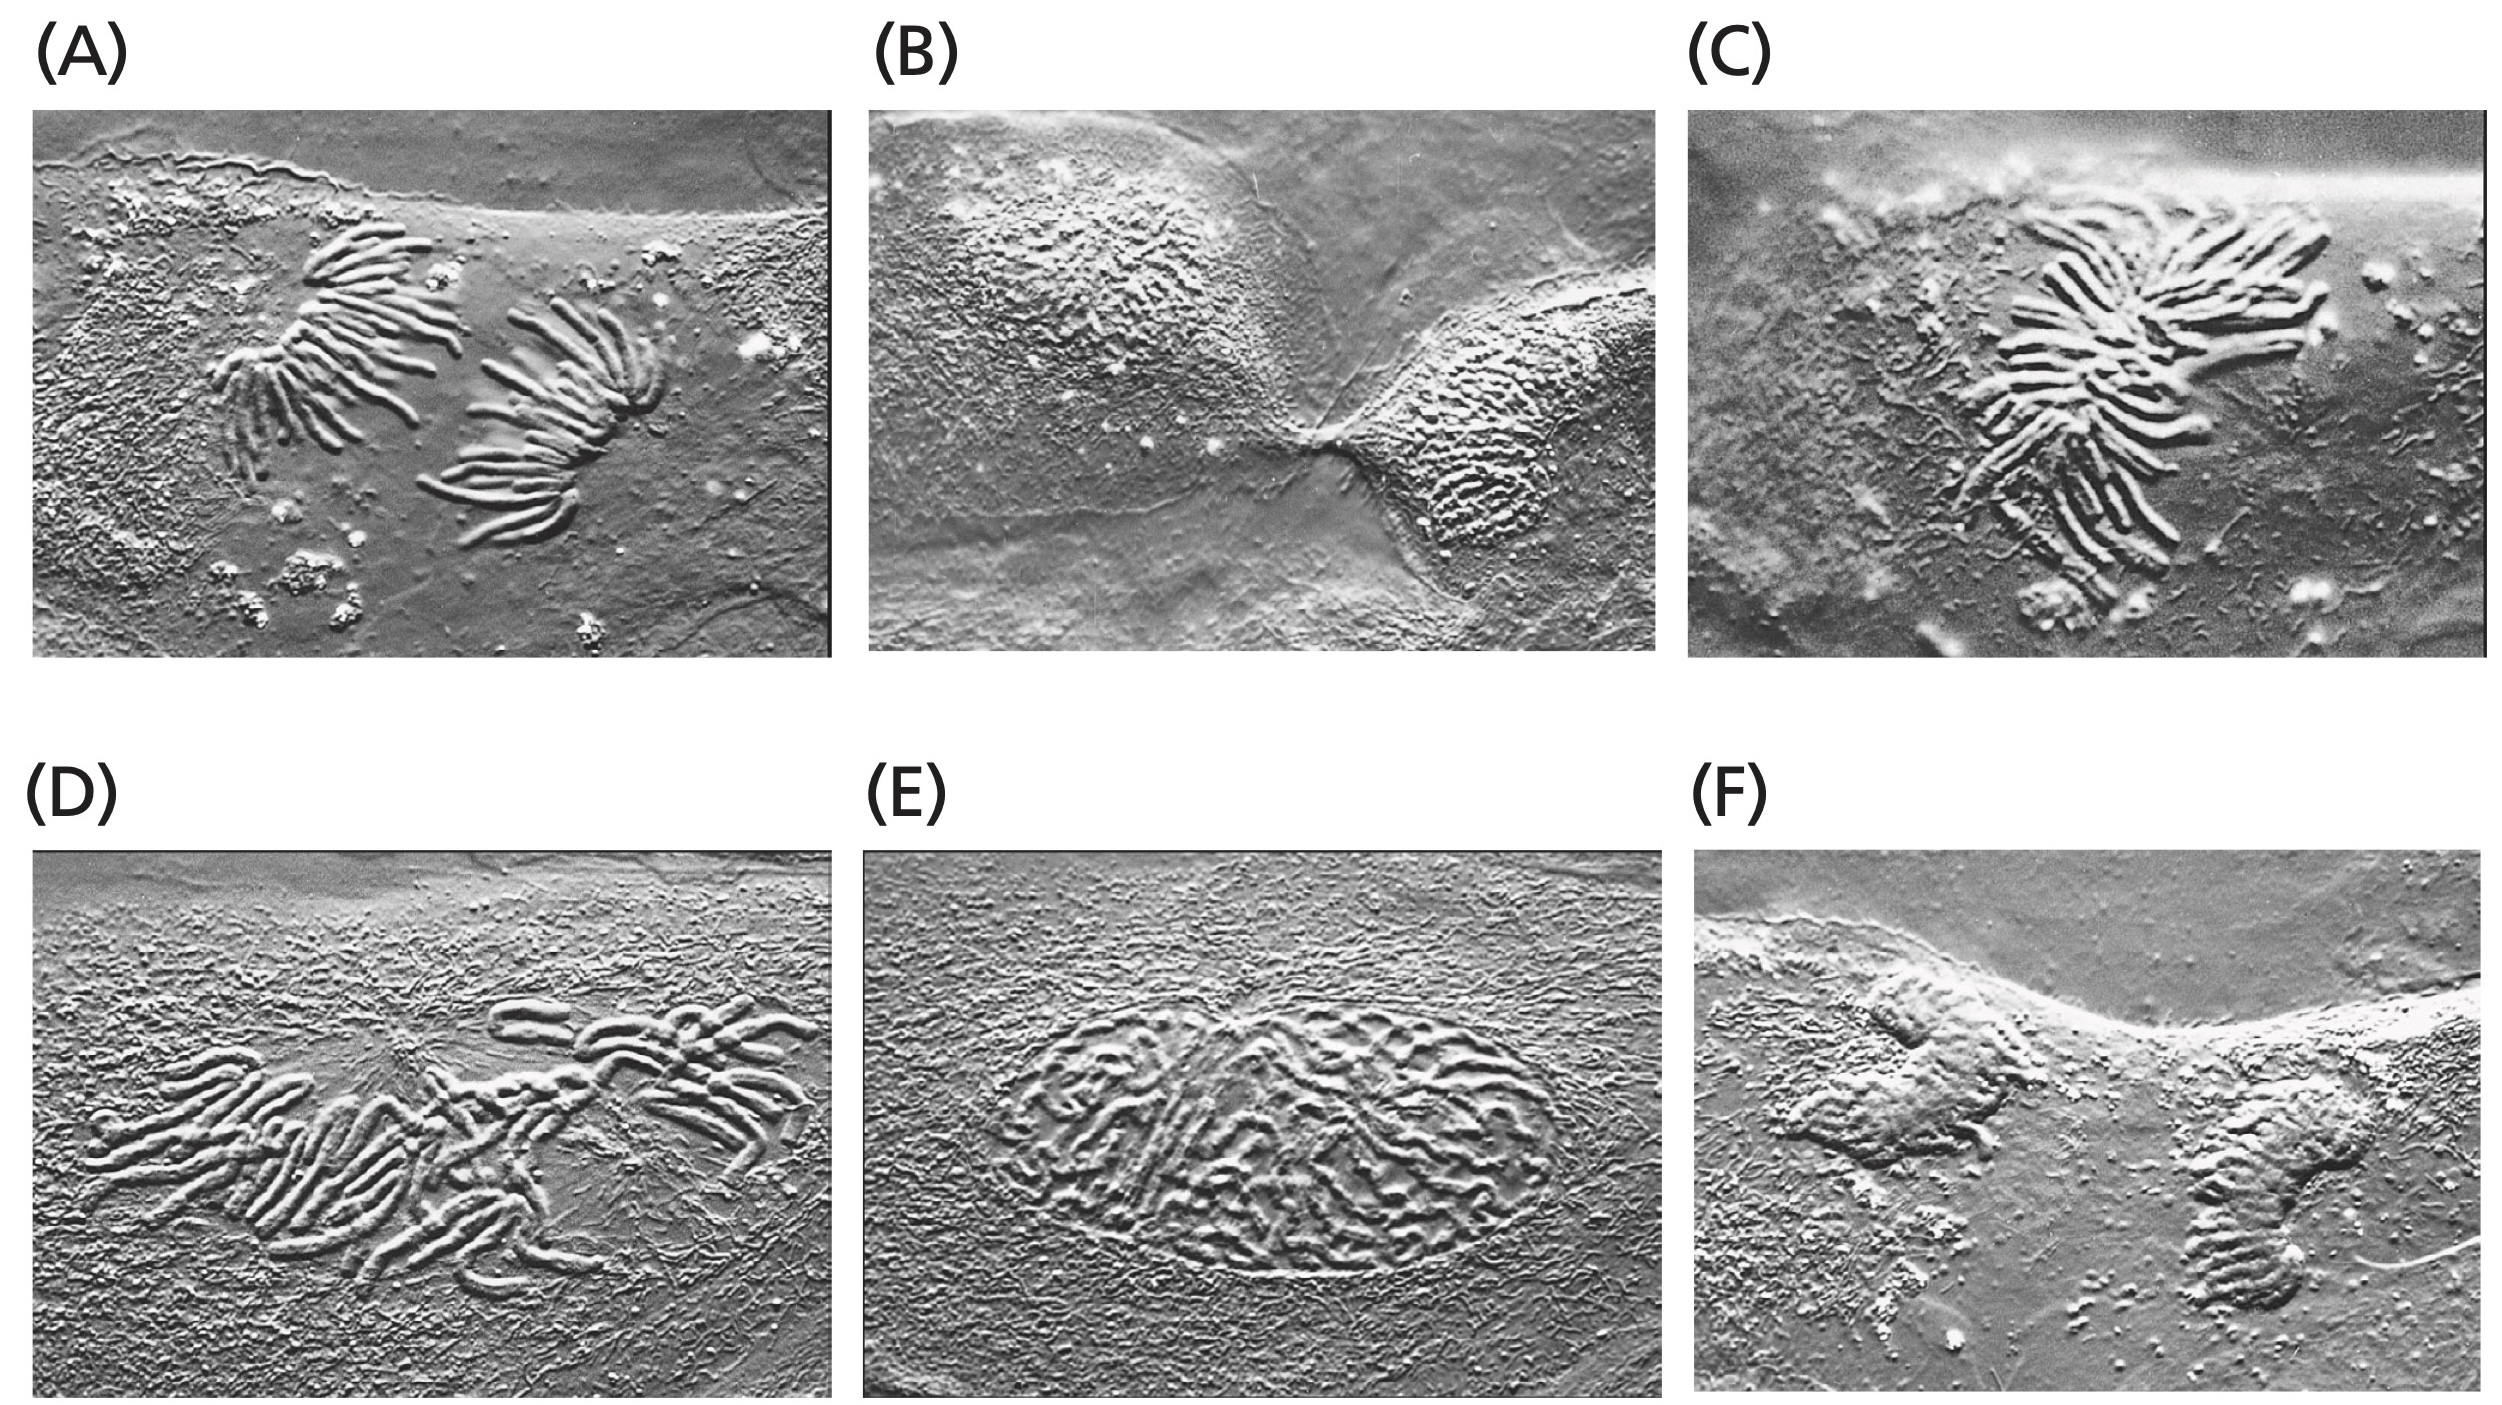
\includegraphics[width = 0.7\linewidth]{Figures/Q17_13.jpg}
    \caption{Q17--13}
\end{figure}
前期 prophase（E），前中期 prometaphase（D），中期 metaphase（C），后期 anaphase（A），末期telophase（F），胞质分裂 cytokinesis（B）。

\subsection{} % Molecular Biology of the Cell 17-18

在减数分裂过程中，每对同源染色体（包括22对常染色体和1对性染色体）中的父源和母源染色体会随机分离到配子中。对于每一对染色体，配子获得父源或母源染色体的可能性各有两种。由于共有23对染色体，且不考虑重组，因此总的潜在组合数为 \(2^{23} = 8388608\) 种。

\subsection{} % Molecular Biology of the Cell 20-9

11 只来自不同地区的袋獾，它们的肿瘤核型高度相似，说明肿瘤细胞源自同一克隆；而且有一只袋獾在 5 号染色体的正常体细胞中有倒位，但其肿瘤细胞中却没有这一倒位，说明肿瘤不是由它自身细胞转变而来，而是外来肿瘤细胞侵入形成的。如果是病毒或微生物诱导的肿瘤，则每只动物的肿瘤应由自身细胞癌变，染色体重排模式会彼此不同，因此这种疾病不太可能主要是由病毒或微生物感染引起的。综上，袋獾的面部肿瘤并不是每只动物自己独立长出来的，而是由一支获得了寄生能力的未知始祖肿瘤细胞系，在个体之间通过撕咬时的细胞移植方式传播的可传染性克隆癌。

\subsection{} % Molecular Biology of the Cell 20-11

这些携带 Brca1 突变的人，他们的正常细胞是 Brca1\textsuperscript{+}/-−，虽然一条 Brca1 基因突变了，但另一条仍正常，所以同源重组修复（HR）还能工作；当使用 PARP 抑制剂 olaparib 时，单链断裂增多并在复制时变成双链断裂，但正常细胞可以依靠剩余的 BRCA1 通过同源重组来修复这些双链断裂，因此大多不被杀死。相反，在这些人身上形成的肿瘤细胞往往已经丢失了最后一条正常 Brca1 拷贝（即 Brca1\textsuperscript{-}/\textsuperscript{-}），同源重组修复完全失效；此时再用 olaparib 抑制 PARP，单链断裂得不到修复并转化为大量双链断裂，而肿瘤细胞又没有 BRCA1 介导的同源重组，只能不断累积致命 DNA 损伤，最终发生细胞死亡，从而实现对肿瘤的选择性杀伤。

\subsection{} % Molecular Biology of the Cell 21-15

在这个节律系统中，每个细胞内部的 Her7 负反馈回路本身就能产生自发振荡，但在没有 Delta 时，各细胞的振荡只靠自身内部机制运行，受转录和降解速率差异以及噪音影响，振荡相位会逐渐彼此错开，结果就是虽然大家都在振荡，但彼此不同步，导致后续形成的体节边界变得模糊；而 Delta 存在时，Her7 振荡会驱动 Delta 表达的周期性变化，Delta 通过与邻近细胞膜上的 Notch 结合激活其 Notch 通路，从而同步启动邻居细胞的 Her7 转录，相当于细胞之间不断互相“校时”，把相位错配的振荡拉回同一节奏，保持相邻细胞振荡同步，因此体节可以形成清晰、规则的边界，也解释了为什么在后期给一个 Delta 脉冲可以重新恢复局部区域体节形成的正常节律。

\subsection{} % Molecular Biology of the Cell 21-16

当在翅膀前部或后部额外表达 Dpp 时，长出的是一团由外观正常的翅膀细胞组成的额外翅膀组织，因此 Dpp 既需要刺激细胞分裂，产生足够多的细胞，也要刺激细胞生长，使它们保持正常形态。

\subsection{} % Molecular Biology of the Cell 24-7

\subsubsection*{A}
从图 B 可以看出：只有用 1968 毒株的 365–380 号氨基酸片段处理靶细胞时，细胞裂解率很高，说明这一段产生的肽正是被该克隆细胞毒 T 细胞（CTL）识别的抗原肽。1968 或 1934 全长核蛋白基因转染时，只有 1968 株能引发强烈裂解，同样说明表位只存在于 1968 的这一小段序列中。其它肽（345–360、369–382，或来自 1934 株的对应肽段）不能有效增敏靶细胞，是因为实验只使用了一种特定的 CTL，它只表达一种特定的 TCR，识别一段特定的肽序列。如果关键氨基酸被替换，就不能被这个特定 TCR 识别，从而不能形成正确的 MHC-肽-TCR 复合物。

\subsubsection*{B}
虽然 MHC I 分子通常在内质网中装载好肽后再运到细胞表面，但表面上的部分 MHC I 分子会偶尔失去原先的肽，或携带结合力较弱的肽，在高浓度外源短肽存在时，这些空/半空的 MHC I 就可以直接在细胞表面与加入的肽发生结合或进行肽交换。这样，只要靶细胞表面出现了一小部分正确的 MHC I-1968 肽复合物，就能被特异性的 CTL 识别并杀伤。

\end{document}